\documentclass[11pt]{article}

% ---- Packages ----
\usepackage[margin=1in]{geometry}
\usepackage{amsmath}
\usepackage{amssymb}
\usepackage{booktabs}
\usepackage{enumitem}
\usepackage{titlesec}
\usepackage{graphicx}
\usepackage[hidelinks]{hyperref}
\usepackage{xcolor}

% ---- Light formatting ----
\definecolor{moss}{HTML}{758C58}
\titleformat{\section}{\large\bfseries\color{moss}}{\thesection}{0.6em}{}
\titleformat{\subsection}{\normalsize\bfseries}{\thesubsection}{0.6em}{}
\setlist{itemsep=2pt, topsep=4pt}
\setlength{\parskip}{0.4em}
\setlength{\parindent}{0pt}

% ---- Title block ----
\title{\vspace{-1.5em}\textbf{The Preferences Arrive with Supervised Fine-Tuning}\\[0.3em]
\large Phase 3 Results: Staged Attribution of Risk and Framing Behavior Across Post-Training}
\author{J. Blakeslee \\ \small RAND School of Public Policy}
\date{\small AI Sprint Practicum (Course 1012) \\ \small September 2026}

\begin{document}
\maketitle

\hrule
\vspace{0.5em}

\section{Introduction}

This project treats large language models as economic agents and recovers their preference
primitives from their choices. Phase 1 fit a structural discrete-choice model to 1{,}200 controlled
lottery choices from \texttt{claude-haiku-4-5} and found that the model prices the probability of
winning and nearly ignores the size of the prize, with an extreme S-shaped Prelec weighting function
($\gamma = 2.69$). Phase 2 held terminal wealth fixed and varied only the wording, and found a
violation of frame invariance: 40\% versus 10\% gamble-taking on arithmetically identical lotteries,
with a stated-reference loss-aversion estimate of $\lambda = 3.234$ under $\phi = 1$. Both phases
measured a single closed frontier model, and both ended on the same open question. Where do these
properties come from?

Phase 3 answers it by moving to open-weight models whose training stages are public. The identical
Phase 1 and Phase 2 instruments are carried to matched base and post-trained checkpoints from three
families, and choice probabilities are read directly from next-token logits rather than sampled.
The decisive asset is OLMo-2-7B, which ships four public checkpoints along one training path: base,
supervised fine-tuned (SFT), preference-optimized (DPO), and final Instruct. Running the same
instruments across that staircase, in a single elicitation format, turns a coarse base-versus-instruct
contrast into a stage-level attribution.

The headline is that the measured behavioral profile arrives at supervised fine-tuning. SFT moves
dominance compliance from 0.555 to 0.756, moves the frame gap from $+0.099$ to $+0.243$, and moves the
structural fit off the parameter boundary where the base model sits. The two later stages, DPO and the
final Instruct polish, are statistically quiet on the preference parameters. Two further results
complicate any simple story about ``LLM biases.'' Base models barely track value at all, so post-training
appears to install the value-tracking that makes the word ``preferences'' apply, rather than merely
bending preferences already present. And the framing response is family-specific: Haiku suppresses
gambling under loss wording, Qwen amplifies it sharply, OLMo amplifies it moderately, and Llama barely
reacts.

\section{The Result in Plain Language}

An AI model is built in stages. First it is trained on a very large amount of text, producing a base
model: a system that continues text plausibly and has never been taught to answer questions. Then it
is fine-tuned, in several distinct steps, to behave like a helpful assistant. Most published work on
AI decision-making tests only the finished assistant, which cannot tell you whether a quirk came from
reading the internet or from the training that came after. One model family, OLMo-2, publishes a
snapshot after each training step. So we asked the money questions from our earlier phases to the same
model at four points in its life, in identical wording each time, and watched what changed.

Almost everything changed at one step, and it was the first one. The base model was close to
incoherent as an economic decision-maker. Offered a sure \$50 against a sure \$70, no gambling
involved, it picked the larger amount barely more often than a coin flip. The base model does not have
odd preferences; it has no preferences in any usable sense, and is producing a plausible-looking letter
rather than comparing two amounts of money. After supervised fine-tuning, the first and simplest of the
assistant-training steps, it picked the larger amount three quarters of the time and began reacting to
how the choices were worded. The two later steps, the ones built on human preference comparisons,
tightened its accuracy on the easy questions and left its economic behavior where supervised
fine-tuning had put it. That is a surprise, because the later stages are the ones people worry about.
Human feedback enters there, and it is the usual suspect when a model shows a human-like bias. Here the
bias is already in place before that stage begins.

Three other things came out of the same runs. The wording effect from Phase 2 has no single direction
across systems. Claude Haiku became much more cautious when the downside was called a loss. Qwen became
dramatically more willing to gamble under the same wording change. OLMo also became more willing, less
dramatically. Llama hardly noticed. Four systems, four responses to one manipulation. The effect is a
property of how a particular model was trained rather than of AI systems in general, so anyone
reporting a framing bias from one model and calling it a fact about language models is reporting a fact
about that model.

The answer also depends on how you ask, in a way that is model-specific and easy to miss. We put the
same questions to each finished assistant in two standard formats. Qwen behaved sensibly in the chat
format and collapsed into near-total refusal to gamble in the other. OLMo did the reverse. Llama was
roughly stable in both. A study comparing two models in one fixed format may be comparing an engaged
model against one that has checked out. The check is cheap: before analyzing anything, confirm the
model reliably picks \$70 over \$50. If it does not, the rest of its answers are not preferences.

The third came from our reviewer, and it is the most uncomfortable. Experimental economists have a
standard move: rather than guess what a subject wants, tell the subject what to want and pay them for
it. We ran the instruction-only version, telling the models in plain language to be expected-value
maximizers, to multiply payoff by probability and take the larger number. They could not do it.
Compliance with the stated rule never rose above roughly 55\% at any training stage, close to a coin
flip, while the same models followed the part of the instruction requiring no arithmetic almost
perfectly, reaching 100\% on the easy questions. Asked for a harder rule involving a square root, one
model's compliance fell to 12\% with a legible error pattern: it compared the transformed payoffs and
dropped the probability entirely. These models are not refusing to comply. They cannot execute an
arithmetic decision rule in a format demanding an immediate one-letter answer, which limits what this
kind of measurement can claim.

\section{Experimental Design}

\subsection{Instruments, grid, and subjects}
Phase 3 reuses the Phase 1 and Phase 2 instruments without modification. The exported grid
(\texttt{data/phase3\_grid.csv}) holds 1{,}680 design cells: 400 Phase-1 risk cells (40 procedurally
generated contamination-safe gambles $\times$ 5 paraphrase templates $\times$ 2 counterbalanced
orders), 1{,}200 Phase-2 framing cells (the same 40 gambles $\times$ 3 frames $\times$ 5 templates
$\times$ 2 orders), and 80 dominant controls pitting a sure amount against a strictly larger sure
amount. Every model sees byte-identical prompts, so nothing in the cross-model comparison is a
difference in the instrument.

Three families, seventeen runs, 28{,}560 elicited choice probabilities. Qwen2.5-7B (base, Instruct under
both formats); Llama-3.1-8B (base, Instruct under both formats), run once Hugging Face access to the
gated repository was approved; and OLMo-2-1124-7B in four stages (base, SFT, DPO, Instruct) plus Instruct
under the chat format. Six further induced runs cover the OLMo staircase under risk-neutral induction and
Qwen Instruct chat under both induced rules.

\subsection{Elicitation by deterministic logits}
Base models do not follow instructions, so the Phase 1--2 forced-tool-choice harness cannot run on
them. Phase 3 reads the choice probability directly. Each prompt is wrapped in a $k = 4$ few-shot
completion (exemplar answers balanced two A and two B, so no letter prior is induced) or passed through
the model's own chat template, and the full next-token distribution is read at the answer position:
\[
  P(\text{gamble}) = \frac{\sum_{t \in \mathcal{T}_g} P(t)}{\sum_{t \in \mathcal{T}_A} P(t)
  + \sum_{t \in \mathcal{T}_B} P(t)},
\]
where $\mathcal{T}_A$ and $\mathcal{T}_B$ are the candidate answer tokens resolved per tokenizer, with
and without a leading space. The unnormalized A/B mass $\sum_{\mathcal{T}_A} P + \sum_{\mathcal{T}_B} P$
is logged per cell as a compliance diagnostic and cells below 0.20 are excluded. One forward pass per
cell replaces roughly 25 sampled repetitions, because the probability is the quantity the logit
likelihood wants. Runs use 4-bit quantization on a free Colab T4.

This also settles a Phase 1--2 nuisance. Temperature 1.0 sampling was treated there as a choice-error
process, an assumption the earlier phases could not test. Phase 3 involves no sampling anywhere: the
logits are deterministic given the prompt, and all randomness in the design is the randomization the
experimenter controls, namely templates, orders, and the payoff grid.

A base and instruct pair differ in weights and in natural elicitation format at the same time, so a
parameter gap could be an artifact of format. Every instruct model is therefore run under both formats,
its chat template and the identical raw few-shot completion the base model receives. This control was
mandatory by design, and it earned its place (Section~5.4).

\subsection{The induced-valuation arm}
Following the reviewer's first point (Section~4.3), a second arm asserts a utility function instead of
eliciting one. The same 1{,}680 cells are re-run with an instruction prepended: either risk-neutral
expected-value maximization, or expected utility with $u(x) = \sqrt{x}$. Compliance with the induced
optimum is scored by \texttt{analysis/score\_induced.py} as the probability mass placed on the
induced-optimal option, reported on cells where the induced rule clearly separates the two options
($|\ln(\mathrm{EU}_g/\mathrm{EU}_s)| \ge 0.05$) and separately on the dominant controls, where both
rules agree and no arithmetic is required. This is the instruction-only version of Smith's (1976)
induced-value procedure, without the incentive that makes the original work.

\section{Econometric Model and Estimation}

\subsection{Fractional maximum likelihood}
The observed data are probabilities, one per design cell, rather than Bernoulli draws. The Phase 1 and
Phase 2 likelihoods carry over unchanged if the Bernoulli log-likelihood is replaced by the binomial
deviance with the observed probability as the target, the standard fractional-response objective (Papke
and Wooldridge 1996):
\[
  D(\theta) = \sum_{c} \left[ y_c \ln \frac{y_c}{\hat p_c(\theta)}
  + (1 - y_c)\ln \frac{1 - y_c}{1 - \hat p_c(\theta)} \right],
\]
where $y_c$ is the elicited probability of the gamble in cell $c$ and $\hat p_c(\theta)$ is the
structural choice probability. The structural model is the Phase 2 specification: reference-dependent
value $v(x) = (x-\rho)^{\alpha}$ for $x \ge \rho$ and $-\lambda(\rho - x)^{\alpha}$ below, with
$\rho = \phi\cdot\text{anchor}$, Prelec weighting $w(p) = \exp(-(-\ln p)^{\gamma})$, a Fechner noise
term $\mu$, and the position nuisance parameter $\delta$. The Phase 1 risk cells are the anchor-zero
rows of the same likelihood, so one estimator covers both instruments. Fitting is by multi-start
Nelder-Mead under the Phase 2 stated-reference restriction $\phi = 1$, and confidence intervals come
from a nonparametric bootstrap that resamples design cells, which is the design distribution the
experiment actually randomizes over.

Validation gate: the estimator recovers the generating parameters near-exactly on the simulated
probability agent (\texttt{data/phase3\_dryrun.csv}), so the degenerate fits reported below are
properties of the models' choice patterns rather than estimator failures.

\subsection{Model-free quantities and held-out validation}
Two quantities need no structural model and are reported as primary throughout. \textbf{Dominance
compliance} is the mean probability placed on the strictly larger sure amount across the 80 dominant
controls, a per-model, per-format engagement check: a subject that fails it is not expressing
preferences. \textbf{The frame gap} is mean $P(\text{gamble})$ in the mixed frame minus the gain frame
over terminal-wealth-identical lotteries, the Phase 2 headline in probability units. Structural
parameters are reported alongside, with boundary flags, for the reason given in Section~8.

Phase 1 closed on an honest weakness: the structural model essentially tied a probability-only logit on
in-sample fit and lost on BIC. \texttt{analysis/holdout\_validation.py} settles it out of sample. The 40
gamble identifiers are split 30/10, each candidate is fit on the training gambles, and mean per-cell
held-out deviance is evaluated on cells belonging to gambles the fit never saw, over 10 random splits.
Candidates are the structural model, a two-parameter logit in the win probability alone, and the
training-mean constant.

\subsection{Reviewer feedback and design response}
Philip Armour reviewed the Phase 1--2 design memo and returned four points in August 2026. Each is
answered by an element of the design above, and the correspondence is worth stating explicitly because
three of the four changed what this phase reports.

\begin{enumerate}[label=\arabic*.]
  \item \textbf{Induced valuation.} His central point invoked the induced-value tradition: if a stated
  utility function cannot be induced in the subject, elicited ``natural'' preferences rest on weaker
  ground, and if it can, compliance calibrates how far to trust the elicitation. This became the arm in
  Section~3.4, and it lands harder here than in Phase 1, because the OLMo staircase can ask where in
  post-training a model becomes the kind of subject induced-value theory presumes. His harder variant,
  denominating payoffs in a token or computation budget so the stakes are real, is the fall workplan.
  \item \textbf{The $\lambda$-$\phi$ collinearity.} He pointed to Rees-Jones and Wang (2022) on testing
  reference points, a minimally parametric approach to the exact degeneracy Phase 2 hit. It is the
  reading gate for the Phase 2 revision.
  \item \textbf{Temperature and what is being randomized.} He asked whether the model's outputs are
  deterministic given the same prompt. They are, and the Phase 3 readout uses precisely that: no
  sampling anywhere, with the design randomization (templates, orders, payoff grid) supplying the
  distribution the bootstrap resamples. His further ask, sampling decision-maker characteristics from
  CPS or ACS distributions, changes the estimand from the deployed assistant to a simulated population,
  so it belongs as an additional arm rather than a replacement.
  \item \textbf{Out-of-sample prediction.} An emphatic yes, and pure analysis on data already in hand.
  Implemented as Section~4.2; it answers the Phase 1 near-tie (Section~5.7).
\end{enumerate}

The project sits inside the structural behavioral economics tradition DellaVigna (2018) surveys:
estimate the parameters of a behavioral model rather than demonstrate a bias, so magnitudes are
comparable across designs and the identifying assumptions are stated. That is what makes a stage-level
attribution meaningful rather than decorative.

\section{Results}

\subsection{Data inventory and engagement}
All eleven uninduced runs completed with a 0\% exclusion rate and high A/B token mass (medians 0.908 to
1.000), so no model is failing to treat the prompt as an A/B question. The induced runs excluded at most
1.8\% of cells. Table~\ref{tab:inventory} reports the inventory alongside the two model-free quantities,
with the Phase 2 Haiku result as the reference row.

\begin{table}[h]
\centering
\caption{Data inventory and model-free quantities. Each run scores the same 1{,}680-cell grid. A/B mass
is the median unnormalized probability on the answer tokens. Dominance is mean probability on the
strictly larger sure amount over 80 controls. The frame gap is mixed minus gain uptake on
terminal-wealth-identical lotteries.}
\label{tab:inventory}
\begin{tabular}{@{}llccccc@{}}
\toprule
Subject & Format & A/B mass & Dominance & Gain & Mixed & Frame gap \\
\midrule
Qwen2.5-7B base        & fewshot & 0.960 & 0.639 & 0.161 & 0.365 & $+0.203$ \\
Qwen2.5-7B Instruct    & fewshot & 0.995 & 0.680 & 0.000 & 0.001 & $+0.001$ \\
Qwen2.5-7B Instruct    & chat    & 1.000 & 0.927 & 0.267 & 0.893 & $+0.626$ \\
\addlinespace
OLMo-2-7B base         & fewshot & 0.908 & 0.555 & 0.499 & 0.598 & $+0.099$ \\
OLMo-2-7B SFT          & fewshot & 0.982 & 0.756 & 0.308 & 0.551 & $+0.243$ \\
OLMo-2-7B DPO          & fewshot & 0.986 & 0.882 & 0.218 & 0.536 & $+0.318$ \\
OLMo-2-7B Instruct     & fewshot & 0.992 & 0.896 & 0.159 & 0.508 & $+0.349$ \\
OLMo-2-7B Instruct     & chat    & 0.985 & 0.636 & 0.475 & 0.552 & $+0.078$ \\
\addlinespace
Llama-3.1-8B base      & fewshot & 0.961 & 0.623 & 0.431 & 0.531 & $+0.099$ \\
Llama-3.1-8B Instruct  & fewshot & 0.983 & 0.782 & 0.444 & 0.478 & $+0.034$ \\
Llama-3.1-8B Instruct  & chat    & 0.999 & 0.804 & 0.589 & 0.538 & $-0.051$ \\
\addlinespace
\textit{claude-haiku-4-5} (Phase 2) & sampled & --- & 1.000 & 0.398 & 0.096 & $-0.302$ \\
\bottomrule
\end{tabular}
\end{table}

\subsection{Base models barely track value}
All three base models emit answer tokens with high confidence and then fail the easiest question in the
instrument. Dominance compliance is 0.555 for OLMo, 0.623 for Llama, and 0.639 for Qwen, against
Haiku's 1.000 in Phase 2. OLMo base picks the gamble at roughly a coin flip in every frame. The few-shot
wrapper is doing what it was built to do, which is to teach the answer format, and it is not producing
value-tracking behavior.

This reframes the attribution question the phase was designed to ask. The plan was to test whether
post-training bends existing preferences toward or away from human patterns. The base models show there
is little to bend: post-training appears to install most of the value-tracking that makes
``preferences'' a meaningful description of the output at all. A base model at 0.56 dominance
compliance does not have unusual preferences, it has no measurable ones, and any structural parameter
fit to its choices describes a pattern closer to statistical noise than to taste.

\subsection{The staircase: attribution to supervised fine-tuning}
The OLMo-2 stages are the core of the phase. All four checkpoints are elicited under the identical
few-shot format, which is OLMo's well-behaved format (Section~5.4), so the format confound is held fixed
by construction rather than by argument. Table~\ref{tab:stairs} and Figure~\ref{fig:stairs} report the
result.

\begin{table}[h]
\centering
\caption{OLMo-2 training staircase, all elicited under the identical few-shot format
($n = 1{,}680$ cells per stage; structural fit on the 1{,}600 core cells under $\phi = 1$).
$^{*}$ = parameter at its bound, where the value and its bootstrap interval are not trustworthy.}
\label{tab:stairs}
\begin{tabular}{@{}lcccccc@{}}
\toprule
Stage & Dominance & Frame gap & $\lambda$ & $\gamma$ & $\alpha$ & $\delta$ \\
\midrule
Base     & 0.555 & $+0.099$ & $0.018^{*}$ & 1.839 & $1.000^{*}$ & $-0.873$ \\
SFT      & 0.756 & $+0.243$ & 1.142 & 0.378 & 0.061 & $+1.179$ \\
DPO      & 0.882 & $+0.318$ & 1.081 & 0.418 & 0.042 & $+1.073$ \\
Instruct & 0.896 & $+0.349$ & 1.057 & 0.349 & 0.035 & $+1.064$ \\
\bottomrule
\end{tabular}
\end{table}

\begin{figure}[h]
\centering
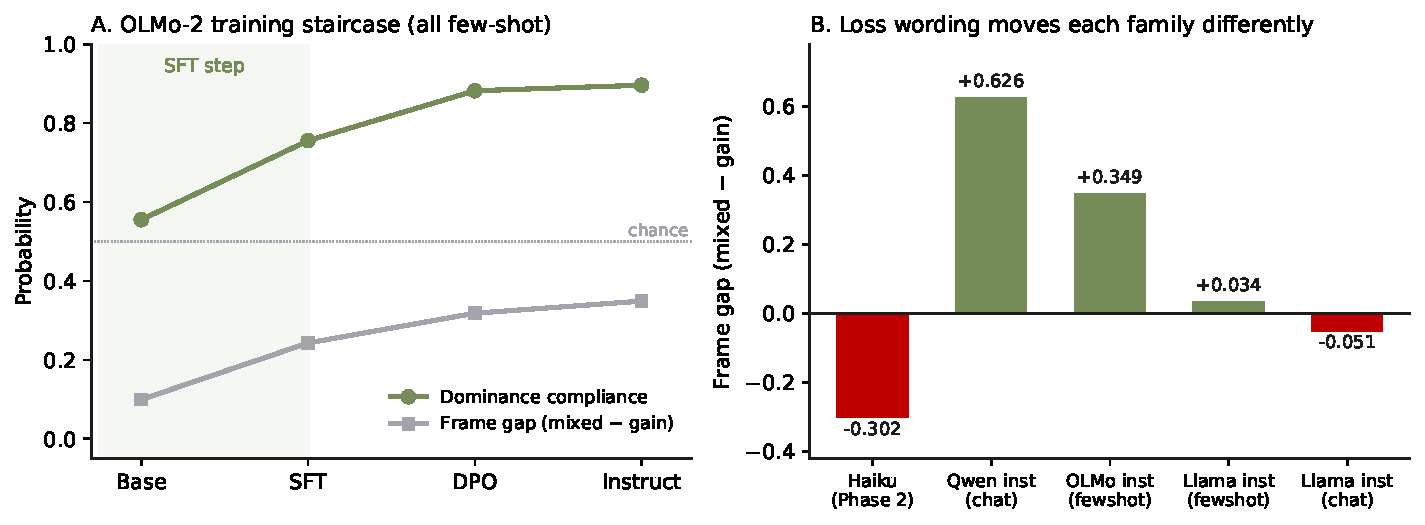
\includegraphics[width=\textwidth]{figures/phase3_staircase.pdf}
\caption{Panel A: the OLMo-2 staircase. Dominance compliance and the frame gap both make their largest
move at supervised fine-tuning, and the base model sits near chance on dominance. Panel B: the framing
response across families, with the Phase 2 Haiku estimate for comparison. The sign and the magnitude
are both family-specific.}
\label{fig:stairs}
\end{figure}

\textbf{Base to SFT: everything moves.} Dominance compliance rises from 0.555 to 0.756. The frame gap
more than doubles, from $+0.099$ to $+0.243$. The structural fit leaves the boundary: $\lambda$ moves off
its lower bound (0.018, at bound) to 1.142, and $\alpha$ moves off its upper bound (1.000, at bound) to
0.061. The position parameter reverses sign, from $-0.873$ to $+1.179$. A base model whose fit sits in a
corner of the parameter space becomes, after one supervised stage, a subject with an interior fit and a
measurable framing response.

\textbf{SFT to DPO: quiet on preferences.} Dominance compliance continues to climb, 0.756 to 0.882, and
the frame gap drifts up to $+0.318$. The preference parameters do not move in a way the bootstrap can
distinguish from zero: $\Delta\lambda = -0.06$ with 95\% CI $[-0.18, +1.06]$, $\Delta\gamma = +0.04$ with
CI $[-0.19, +0.39]$. Preference optimization sharpens compliance on the unambiguous questions without
relocating the estimated preference.

\textbf{DPO to Instruct: quiet throughout.} Dominance 0.882 to 0.896, frame gap $+0.318$ to $+0.349$,
$\Delta\lambda = -0.02$ with CI $[-0.14, +0.11]$, $\Delta\gamma = -0.07$ with CI $[-0.26, +0.17]$,
$\Delta\alpha = -0.01$ with CI $[-0.11, +0.14]$. Every interval covers zero.

The attribution localizes to supervised fine-tuning. Stated as the phase's central claim: in this
family, on these instruments, the behavioral profile measured in the instruction-tuned model is already
fully present after supervised fine-tuning, and the preference-based stages neither add it nor remove
it. This matters because preference-based post-training, the stage where human feedback enters, is the
usual suspect in the literature that attributes cognitive biases to instruction tuning (Itzhak et al.
2024). Here the suspect has an alibi.

\subsection{Format instability, with a model-specific direction}
The dual-format arm was included as a control and returned a result. The same Qwen Instruct weights
behave as two different subjects under the two formats. In the chat format it reaches 0.927 dominance
compliance and a $+0.626$ frame gap. In the few-shot format it refuses the gamble almost totally (uptake
0.000 in the gain frame, 0.001 in the mixed frame), the frame gap vanishes, the structural $\lambda$
pins at its upper bound of 54.6, the same corner the free-$\phi$ Phase 2 fit slid into, and
$\delta = -4.67$, which says the choices are riding position rather than value.

OLMo Instruct shows the same instability in the opposite direction. Few-shot is its well-behaved format
(dominance 0.896, frame gap $+0.349$); the chat format degrades it (dominance 0.636, frame gap $+0.078$,
$\delta = +3.83$). Llama Instruct is the exception that makes the pattern legible: it is roughly stable
across both formats, with dominance 0.782 few-shot and 0.804 chat, and frame gaps of $+0.034$ and
$-0.051$.

Two methodological consequences follow. Format instability generalizes across model families, while
which format elicits engaged behavior does not. And a cross-model comparison must hold format fixed
\emph{and} verify per model that the fixed format elicits engagement, or it risks comparing an engaged
model against one that has disengaged. Dominance compliance is the cheap check, at 80 cells per model
per format. The OLMo staircase in Section~5.3 is all-few-shot, OLMo's good format, so the staged
attribution is unaffected.

The same finding disqualifies one contrast the phase set out to run. The Qwen base-to-instruct
attribution under the few-shot format ($\Delta\lambda$ CI $[+3.6, +53.7]$, $\Delta\gamma$ CI
$[+0.71, +1.25]$) cannot be read as a post-training effect, because the instruct model's few-shot
behavior does not represent that model in its natural format; it is reported as format-confounded and
excluded from the attribution claims. The Llama pair, elicited few-shot on both sides of a format-stable
instruct model, gives $\Delta\lambda = +1.18$ with CI $[+1.05, +1.25]$ and $\Delta\gamma = -0.98$ with
CI $[-1.65, -0.71]$ from base to instruct, with the usual caveat that the base fit is boundary-pinned.

\subsection{Framing heterogeneity across families}
Phase 2 found that Haiku suppresses gambling under loss wording, a frame gap of $-0.302$, which runs
against the textbook prospect-theory direction of risk-seeking in the domain of losses. Every open model
here moves the other way or barely moves. Qwen Instruct in chat amplifies strongly, $+0.626$. The OLMo
stages amplify moderately, $+0.24$ to $+0.35$. Llama Instruct is nearly frame-invariant, $+0.034$
few-shot and $-0.051$ chat.

Three families, three responses to the identical manipulation, and a fourth from the frontier model in
Phase 2. The cross-model heterogeneity is a stronger result than any single family's gap. Loss framing
is not a fixed property of language models as a class, and the direction of the response is plausibly a
function of the post-training recipe. A literature that estimates a prospect-theory parameter on one
instruct model and reports it as a fact about LLMs is over-generalizing from a sample of one recipe. The
staircase supplies the complementary within-family fact: framing sensitivity is installed early, then
grows monotonically but modestly through the later stages.

\subsection{Induced valuation: the models cannot execute an induced rule}
Table~\ref{tab:induced} reports compliance with an explicitly instructed decision rule.

\begin{table}[h]
\centering
\caption{Induced-valuation compliance under a risk-neutral expected-value instruction. Compliance is the
mean probability mass on the induced-optimal option, restricted to cells where the induced rule clearly
separates the options ($|\ln \mathrm{EU}$ ratio$| \ge 0.05$; 1{,}221 to 1{,}240 cells per run). Baseline
is the uninduced run from the same model and format, scored against the same rule.}
\label{tab:induced}
\begin{tabular}{@{}lccccc@{}}
\toprule
 & \multicolumn{3}{c}{EV compliance, clear cells} & \multicolumn{2}{c}{Dominance compliance} \\
\cmidrule(lr){2-4}\cmidrule(lr){5-6}
Subject (format) & Baseline & Induced & Difference & Baseline & Induced \\
\midrule
Qwen Instruct (chat)  & 0.524 & 0.541 & $+0.017$ & 0.927 & 0.886 \\
OLMo base (fewshot)   & 0.516 & 0.545 & $+0.029$ & 0.555 & 0.593 \\
OLMo SFT (fewshot)    & 0.493 & 0.525 & $+0.032$ & 0.756 & 0.821 \\
OLMo DPO (fewshot)    & 0.470 & 0.533 & $+0.063$ & 0.882 & 0.950 \\
OLMo Instruct (fewshot) & 0.449 & 0.524 & $+0.075$ & 0.896 & 0.969 \\
\bottomrule
\end{tabular}
\end{table}

Instruction-only induction fails on cells requiring computation, at every training stage, in both
families. Compliance mass on expected-value-clear cells never exceeds roughly 0.55 anywhere, close to
indifference. The induction effect grows monotonically up the OLMo staircase (from $+0.017$ to $+0.073$
on all core cells, $+0.029$ to $+0.075$ on clear cells) and stays trivial in absolute terms. Instructed
dominance compliance moves the opposite way, climbing to 0.950 and 0.969 in probability mass at the DPO
and Instruct stages, which is 1.000 in hard accuracy: every dominant control answered correctly.

The instruction helps exactly where the induced optimum requires no arithmetic and does nothing where it
requires multiplying $p$ by $h$. The sharpest evidence is the square-root run. Told that
$u(x) = \sqrt{x}$, Qwen Instruct's compliance collapsed to 0.124 hard accuracy on clear cells, far below
its own uninduced 0.479, and the errors have a legible pattern: gain-frame accuracy of 0.035 corresponds
to near-always gambling, which is what comes of comparing square-root-transformed payoffs while dropping
the probability term. The model did something with the instruction. It did not do the instruction.

This supports ``cannot compute in this format'' over ``will not comply.'' In an immediate-answer
elicitation the model must emit a letter at the next token with no intermediate computation available,
while post-training steadily improves its following of the no-computation part of an instruction. The
induced-value calibration therefore returns a negative result, and the negative result is informative:
it puts a ceiling on how much any immediate-answer elicitation of this kind can claim about deliberate
optimization. The decisive follow-up is a reason-then-answer induced arm that lets the model compute the
expected value before committing to a letter. That arm is not in this phase, so until it runs, the
inability reading is the better-supported one rather than the proven one.

\subsection{Held-out validation}
Phase 1 reported honestly that a probability-only logit essentially tied the structural model in sample
and beat it on BIC. It does not survive out of sample. Fitting on 30 gambles and predicting cells from
the 10 held-out gambles, over 10 random splits, the structural model wins on every split for all three
families tested. Mean held-out per-cell deviance is 0.297 for the structural model against 0.401 for the
probability-only logit and 0.411 for the constant on Qwen Instruct chat; 0.285 against 0.333 and 0.345 on
OLMo Instruct few-shot; and 0.094 against 0.117 and 0.125 on Llama Instruct few-shot. The tally is 10/10
splits in each family, and the ordering is the same on root mean squared error.

The structural model therefore earns its place on prediction, not on interpretability alone. Win
probability explains a great deal of the behavior, as Phase 1 found. It does not explain the behavior on
gambles the fit has never seen.

\section{Interpretation}

\textbf{Post-training creates the subject before it shapes the taste.} The intuitive picture of a base
model with raw preferences that alignment then bends is not what the data show. Base models fail the
dominance control at 0.56 to 0.64 while emitting answer tokens confidently, which is a subject producing
a plausible letter rather than comparing two amounts of money. Whatever economic behavior is measurable
in the instruct models is largely built during post-training rather than inherited and adjusted. Asking
where a bias came from presupposes that something was there to be biased.

\textbf{Supervised fine-tuning is where it happens, and that is a surprise.} Preference-based training
is the stage most often blamed for human-like biases, since it is the stage where human judgments enter
the weights. In the one family that publishes stage-level checkpoints, the frame gap, the value-tracking,
and the interior structural fit are all in place after supervised fine-tuning, and DPO and the final
polish move nothing the bootstrap can detect. The intervals are wide enough that a small later-stage
effect cannot be excluded, and this is one family with one set of instruments. Yet the ordering is clear,
and it points research attention at the least glamorous stage.

\textbf{The bias is a property of a recipe rather than of a technology.} Four systems, four responses to
the same loss-wording manipulation, from strong suppression through strong amplification to near
indifference. The published work reporting prospect-theory parameters for a single instruction-tuned
model, including the closest incumbents (Liu et al. 2025; arXiv:2508.08992), is describing a training
recipe. Heterogeneity of this size means an evaluation performed on one model transfers to another only
by assumption.

\textbf{Format is a measurement instrument, and it is not neutral.} The same weights produced a coherent
economic subject and a near-total gambling refusal depending only on whether the prompt arrived as a
chat message or a raw completion, and which format worked reversed between families. Any benchmark
comparing models under one fixed format is running an uncontrolled interaction.

\textbf{The elicitation has a ceiling, and the induced arm found it.} The models cannot follow an
instructed arithmetic decision rule in this format while following the non-arithmetic part of the same
instruction perfectly. That constrains the reading of every structural parameter in Phases 1 through 3.
These are parameters of an immediate-answer choice process rather than of a deliberate optimization the
model is capable of and chose to depart from. The restriction on the estimand is real, and more useful
stated than assumed away. Phase 2's free-$\phi$ degeneracy also reappeared here, as Qwen's few-shot
$\lambda$ pinned at 54.6, the identical corner of the identical likelihood surface reached by a different
route, which marks it as a property of the specification rather than of any one subject.

\section{Policy Relevance}

\textbf{The attribution has an intervention point.} If a behavioral property is installed at supervised
fine-tuning, the place to inspect, audit, or correct it is the supervised data and the checkpoint that
immediately follows, rather than the preference-optimization stage that receives most of the governance
attention. The method generalizes: any lab retaining intermediate checkpoints can run this diagnostic on
any behavioral property a fixed instrument can measure.

\textbf{Stage-level attribution requires open checkpoints, which is a policy variable.} The result exists
because one organization published four checkpoints along its training path. No frontier developer does.
An evaluation regime that wants to attribute model behavior to training decisions, rather than only
document that the behavior exists, depends on staged-checkpoint access for auditors. That access is a
policy choice available now, and it is inexpensive relative to what it buys.

\textbf{Evaluations need engagement checks or they will report randomness as preference.} Two results here
are ways a plausible-looking evaluation goes wrong. A base model returns confident answer tokens and
coherent-looking parameters while failing to prefer \$70 to \$50. An instruct model returns a completely
different economic profile under a different prompt format. Both produce publishable-looking numbers,
and 80 dominance controls catch both. Any evaluation regime for agentic systems should require the
engagement diagnostic alongside the headline, for the same reason a survey reports its response rate.

\textbf{Do not port a measured bias across models.} An agent that suppresses risk-taking under loss
wording and one that amplifies it will move in opposite directions on the same procurement menu, the
same insurance framing, the same triage prompt. A framing vulnerability documented on one model tells a
procurement officer nothing reliable about the model deployed, so the measurement must be repeated per
model. That is the argument for cheap standardized instruments of the kind this project builds.

\textbf{Scope.} These are properties of specific open-weight checkpoints under a deterministic logit
readout with unincentivized forced choice. They are not claimed as universal traits of language models,
and the framing-heterogeneity result is precisely the reason such claims are unsafe.

\section{Limitations and Next Phase}

\textbf{Boundary-pinned structural fits.} The base-model and Qwen-instruct-few-shot fits sit at parameter
bounds ($\lambda$ at 0.018 or 54.6, $\alpha$ at 1.0). Values at a bound are not trustworthy and neither
are their bootstrap intervals; one interval in the base-to-SFT contrast overflowed outright. Model-free
quantities are therefore primary throughout, structural fits carry boundary flags, and a wider-bounds
refit with profile-likelihood intervals is the correct next step for every contrast touching a base
model. The staircase's qualitative claim does not depend on the pinned values, since the move at SFT is
visible in dominance compliance and the frame gap alone.

\textbf{One instruction phrasing in the induced arm.} Each induced rule was tested under a single
phrasing. A compliance failure under one phrasing is weaker evidence than a failure under several, and
the robustness check is unrun.

\textbf{The immediate-answer format cannot separate inability from unwillingness.} This is the sharpest
open question the phase raises about its own method. The reason-then-answer induced arm is the decisive
test and belongs at the top of the follow-on list, next to the token-budget incentive-compatible design
that would make the induced-value procedure complete rather than instruction-only.

\textbf{Hardware, quantization, and one staircase.} All runs use 4-bit quantization on free Colab T4
hardware. The exercise compares checkpoints under identical conditions, so a small uniform quantization
effect would not disturb the staircase, though this is unverified against full precision. The
stage-level attribution also rests on one family, because OLMo-2 is the only family publishing
intermediate checkpoints. A second staged family would turn the central claim into a replication.

Phase 3 has done its job. It carries the Phase 1 and Phase 2 instruments to models whose training history
is visible, localizes the measured behavioral profile to supervised fine-tuning, shows that base models
lack the value-tracking that would make the word ``preference'' apply, documents that the framing response
differs in sign across families, and answers the Phase 1 near-tie out of sample. It also found the ceiling
of its own elicitation, which the next phase should raise before adding new instruments to it.

\vspace{1em}
\hrule
\vspace{0.5em}

\begin{thebibliography}{99}
\small

\bibitem{dellavigna2018}
DellaVigna, S. (2018).
Structural Behavioral Economics. In \textit{Handbook of Behavioral Economics}, Vol.\ 1, 613--723;
NBER Working Paper 24797.

\bibitem{holt2002}
Holt, C. A., and Laury, S. K. (2002).
Risk Aversion and Incentive Effects. \textit{American Economic Review}, 92(5), 1644--1655.

\bibitem{itzhak2024}
Itzhak, I., Stanovsky, G., Rosenfeld, N., and Belinkov, Y. (2024).
Instructed to Bias: Instruction-Tuned Language Models Exhibit Emergent Cognitive Bias.
\textit{Transactions of the ACL}; arXiv:2308.00225.

\bibitem{kahneman1979}
Kahneman, D., and Tversky, A. (1979).
Prospect Theory: An Analysis of Decision under Risk. \textit{Econometrica}, 47(2), 263--291.

\bibitem{koszegi2006}
K\H{o}szegi, B., and Rabin, M. (2006).
A Model of Reference-Dependent Preferences. \textit{Quarterly Journal of Economics}, 121(4), 1133--1165.

\bibitem{liu2025}
Liu, J., Yang, Y., and Tam, K. Y. (2025).
Evaluating and Aligning Human Economic Risk Preferences in LLMs.
\textit{Proceedings of EMNLP 2025}; arXiv:2503.06646.

\bibitem{cpt2025}
CPT Estimation on LLMs (2025). Cumulative Prospect Theory Parameters of Instruction-Tuned Language
Models. arXiv:2508.08992.

\bibitem{papke1996}
Papke, L. E., and Wooldridge, J. M. (1996).
Econometric Methods for Fractional Response Variables. \textit{Journal of Applied Econometrics},
11(6), 619--632.

\bibitem{prelec1998}
Prelec, D. (1998).
The Probability Weighting Function. \textit{Econometrica}, 66(3), 497--527.

\bibitem{reesjones2022}
Rees-Jones, A., and Wang, K. (2022).
An Approach to Testing Reference Points. NBER Working Paper 30773.

\bibitem{smith1976}
Smith, V. L. (1976).
Experimental Economics: Induced Value Theory. \textit{American Economic Review}, 66(2), 274--279.

\bibitem{train2009}
Train, K. E. (2009).
\textit{Discrete Choice Methods with Simulation} (2nd ed.). Cambridge University Press.

\bibitem{tversky1981}
Tversky, A., and Kahneman, D. (1981).
The Framing of Decisions and the Psychology of Choice. \textit{Science}, 211(4481), 453--458.

\bibitem{tversky1992}
Tversky, A., and Kahneman, D. (1992).
Advances in Prospect Theory: Cumulative Representation of Uncertainty.
\textit{Journal of Risk and Uncertainty}, 5(4), 297--323.

\bibitem{wu1996}
Wu, G., and Gonzalez, R. (1996).
Curvature of the Probability Weighting Function. \textit{Management Science}, 42(12), 1676--1690.

\end{thebibliography}

\end{document}
